\documentclass[pdftex,a4paper,12pt]{article}
\usepackage[T2A]{fontenc}
\usepackage[russian]{babel}
\usepackage{ucs}
\usepackage[utf8]{inputenc}
\usepackage{graphicx}
\usepackage[font=small,labelfont=bf]{caption}
\usepackage[unicode=true]{hyperref}
\hypersetup{
		pdftitle={Богданов Д.А., “Численное исследование течения в фильтре-циклоне”, 2012},
    colorlinks,
    citecolor=black,
    filecolor=black,
    linkcolor=black,
    urlcolor=black
}
\title{Численное исследование течения в фильтре-циклоне}
\author{Дмитрий Богданов}
\date{}
\begin{document}
\begin{titlepage}
	\begin{center}
		\small{МИНИСТЕРСТВО ОБРАЗОВАНИЯ И НАУКИ \\ РОССИЙСКОЙ ФЕДЕРАЦИИ \\
Санкт-Петербургский государственный политехнический университет \\
Физико-механический факультет \\
Кафедра гидроаэродинамики}\\
		\vspace{0.05\textheight}
	\end{center}
	\begin{flushright}
		\normalsize
			Диссертация допущена к защите \\
			Зав. кафедрой, проф., д.ф-м.н.\\
			\underline{\hspace{7em}} Е.М. Смирнов \\
			"\underline{\hspace{2em}}" \underline{\hspace{9em}} 2012г. \\
	\end{flushright}
	\begin{center}
		\vspace{0.1\textheight}
		\large{Численное исследование течения в фильтре-циклоне}\\
		\vspace{0.01\textheight}
		\normalsize
		\textsc{Диссертация на соискание ученой степени магистра по направлению 010600 – Прикладные математика и физика}
		\vspace{0.25\textheight}
	\end{center}
	\begin{minipage}{0.48\textwidth}
		\begin{flushleft}
			Выполнил студент гр. 6054/11\\
			Руководитель, к.ф.-м.н., доц.\\
		\end{flushleft}
	\end{minipage}
	\begin{minipage}{0.5\textwidth}
		\begin{flushright}
			Богданов Д.А. \\
			Поняев С.А. \\
		\end{flushright}
	\end{minipage}
	\vspace{0.1\textheight}
	\begin{center}
		Санкт-Петербург \\
		\the\year
	\end{center}
\end{titlepage}
\newpage

\tableofcontents
\newpage
\section{Введение}
	\subsection{Актуальность проблемы}
		\hspace{2em} 	Задача очищения атмосферного воздуха от загрязняющих выбросов промышленных предприятий достаточно актуальна. Выбросы от стационарных источников вредных веществ в атмосферу городов и населенных пунктов, расположенных на территории северо-западного федерального округа,  по данным Росстата за 2007 год,  составили 2319000 тонн, в том числе твёрдых -- 289400 тонн \cite{emissionInfoRussian}.
		\begin{figure}[ht]
			\vspace{-1em}
			\begin{minipage}[b]{0.46\linewidth}
				В некоторых отраслях промышленности доля выбросов пыли в атмосферу достигает 15\% от общего числа получаемого продукта. Так, при изготовлении одной тонны цемента в воздух выбрасывается $\approx 160$ кг цементной пыли \cite{emissionInfoEurope}.
				Динамика изменения объёма выбросов твёрдых вредных веществ в атмосферу \textit{(рис. \ref{figure:atmosphereDynamic})} имеет тенденцию к росту, что говорит о том, что решение проблемы инженерной защиты воздуха от вредных веществ останется актуальной и в ближайшем будущем. 
			\end{minipage}
			\hspace{0.01\linewidth}
			\begin{minipage}[b]{0.48\linewidth}
				\centering
				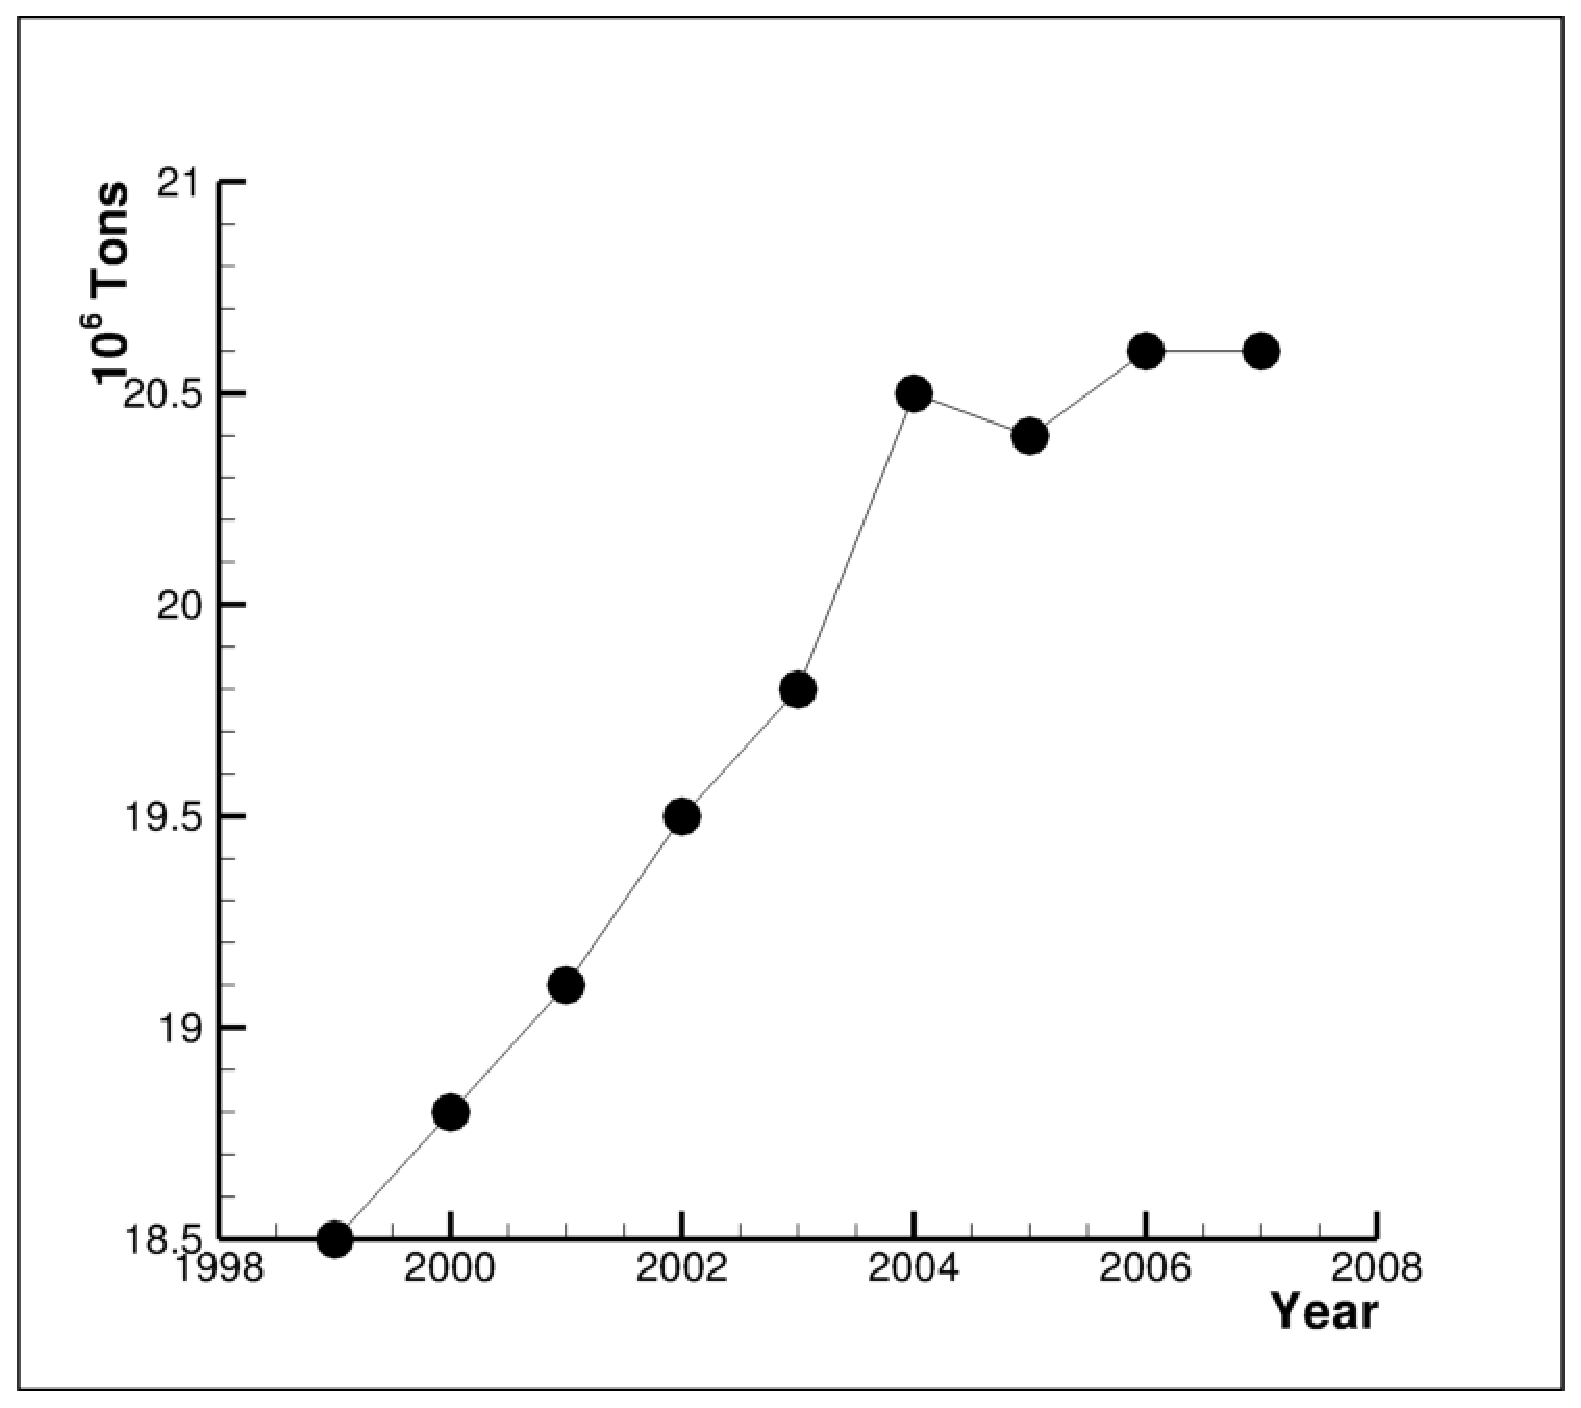
\includegraphics[scale=0.24]{atmosphereDynamic}
				\caption{Динамика выбросов твёрдых вредных веществ в атмосферу \cite{emissionInfoRussian}}
				\label{figure:atmosphereDynamic}
			\end{minipage}
		\end{figure}
		\vspace{-1em}
	
		Для очищения воздуха от твёрдых примесей широкое распространение получили фильтры типа циклон. Циклон представляет собой инерционный пылеуловитель, в котором выделение частиц из воздушной среды происходит, в основном, под действием центробежной силы, возникающей при вращении воздушного потока в корпусе аппарата.
	
		Запылённый воздух входит в циклон через тангенциальный патрубок и, приобретая вращательное движение, опускается винтообразно вниз вдоль внутренних стенок цилиндра и конуса. Небольшая часть этого потока, в котором сконцентрированы пылевые частицы, движется в непосредственной близости от стенок циклона и поступает через пылеотводящее отверстие в пылесборный бункер, где происходит осаждение и накопление пылевых частиц.
	
		В центральной зоне циклона воздушный поток, освобождённый от пыли, поднимается винтообразно вверх и удаляется через выхлопную трубу наружу.
	
		Вследствие вращательного движения воздушного потока в центральной зоне циклона (в конусе, выхлопной трубе и пылесборном бункере) наблюдается пониженное давление.\cite{instructions}
	
		В силу высокой степени закрученности потока, необходимо введение поправок в модели турбулентности для учёта кривизны линий тока. Кроме того, учитывая высокую концентрацию частиц в потоке, в инженерных расчётах необходимо учитывать не только влияние потока на частицы, но также и обратное влияние частиц на поток.
	%Актуальность проблемы
	\subsection{Цели работы}
		\begin{enumerate}
			\item Реализация $k-\omega-SST$ модели турбулентности с поправкой на кривизну линий тока при помощи открытой интегрируемой платформы для численного моделирования задач механики сплошных сред OpenFOAM.
			\item Реализация с использованием OpenFOAM солвера, имеющего в основе модель идеального газа и учитывающего при этом обратное влияние частиц на поток.
			\item Численное моделирование циклона с учётом обратного влияния частиц на поток и поправки на кривизну линий тока к генерации турбулентности.
		\end{enumerate}
	%Цели работы
\newpage
%Введение

\section{Обзор существующих исследований}
	\subsection{Экспериментальные исследования}
		\hspace{2em}Существует большое количество работ по экспериментальному исследованию течения с криволинейными линиями тока. Среди них стоит выделить достаточно подробный эксперимент, приведённый в статье Monson et al. \cite{Monson}. Авторы статьи проводят численное и экспериментальное исследование турбулентного течения воздуха в U-образном канале.
	
		Экспериментальному моделированию циклонов также уделено немало внимания. Среди статей, приводящих экспериментальные данные по турбулентному течению в циклонах, нужно отметить детальное исследование течения в циклоне модели Stairmand, описанное в статье J. Dirgo, D. Leith \cite{DirgoLeith}. В этой статье приведены данные для профилей скорости в нескольких сечениях фильтра для большого диапазона рабочих параметров. К сожалению!!!!!!!!!!!!!!!!!!!!!!!!!!!1
	\subsection{Теоретические исследования}
		\hspace{2em}Среди теоретических исследований течения в циклонах особо выделим статью 
	\subsection{Численные исследования}
		\hspace{2em}Численному моделированию течения в циклонах посвящено очень много инженерных исследований.
	%Численные исследования
\newpage
%Обзор существующих моделей
\section{Численное моделирование}
	\subsection{OpenFOAM}

		\hspace{2em}OpenFOAM — свободно распространяемый инструментарий вычислительной гидродинамики для операций с полями (скалярными, векторными и тензорными). На сегодняшний день является одним из самых известных приложений с открытым кодом, предназначенных для FVM-вычислений.\cite{openfoam}
		Код OpenFOAM, разработан в Великобритании в компании \textit{OpenCFD, Limited}, и используется многими промышленными предприятиями более 12 лет. Свое название и идеологию построения код берет от предшественника FOAM (Field Operation And Manipulation), который является закрытым и продолжает развиваться параллельно с OpenFOAM. Первоначально, программа предназначалась для прочностных расчетов и в результате многолетнего академического и промышленного развития на сегодняшний момент позволяет решать следующие задачи:
	\begin{itemize}
		\item Прочностные расчеты;
		\item Гидродинамика сжимаемых и несжимаемых сред. Для моделирования турбулентных течений возможно использование RANS и LES - методов. Возможно решение дозвуковых, околозвуковых и сверхзвуковых задач;
		\item Задачи теплопроводности в твёрдом теле;
		\item Течения многофазных сред;
		\item Течения химически реагирующих смесей;
		\item Задачи, связанные с деформацией расчётной сетки;
		\item Распараллеливание расчёта как в кластерных, так и многопроцессорных системах.
	\end{itemize}

	В основе кода лежит набор библиотек, предоставляющих инструменты для решения систем дифференциальных уравнений в частных производных. Рабочим языком кода является C++. В терминах данного языка большинство математических операторов в программном коде уравнений может быть представлено в удобочитаемой форме, а метод дискретизации и решения для каждого оператора может быть выбран уже пользователем в процессе расчёта. Таким образом, в коде полностью инкапсулируются и разделяются понятия расчетной сетки, дискретизации основных уравнений и методов решения алгебраических уравнений.
	%OpenFOAM
	\newpage
	\subsection{Метод конечных объёмов \cite{OPNFPG}}
		\subsubsection{Дискретизация расчётной области}
			Суть метода конечных объёмов 
		\subsubsection{Дискретизация уравнений}
			Дискретизация уравнений преобразует уравнения в частных производных в систему алгебраических уравнений, которые обычно представляются в виде матричной форме:
			\begin{equation}
				[A][x] = [B],
			\end{equation}
			где [A] - квадратная матрица, [x] - столбец неизвестных, а [B] - 
	%Метод конечных объёмов
	\newpage
	\subsection{Основные уравнения}
		\subsubsection{Уравнение баланса массы}
			\begin{equation}
				\frac{\partial \rho}{\partial t} + \frac{\partial}{\partial x_i}(\rho u_i) = 0
			\end{equation}
		\subsubsection{Уравнение баланса импульса}
			\begin{equation}
				\frac{\partial \rho u_i}{\partial t} + \frac{\partial}{\partial x_j}(\rho u_iu_j) = - \frac{\partial p}{\partial x_i} + \frac{\partial {\tau_{ij}}_{eff}}{\partial x_j},
			\end{equation}
			где ${\tau_{ij}}_{eff}$ - тензор вязких напряжений, выражаемый по формуле
			\begin{equation}
				{\tau_{ij}}_{eff} = \mu_{eff}\left( \frac{\partial u_i}{\partial x_j} + \frac{\partial u_j}{\partial x_i} \right) - \frac{2}{3}\mu_{eff}\frac{\partial u_i}{\partial x_j} \delta_{ij} \quad \mu_{eff} = \mu + \mu_{t}
			\end{equation}
		\subsubsection{Уравнение баланса энтальпии}
		\subsubsection{Уравнение состояния}
			\hspace{2em}При расчётах течений сжимаемой жидкости используется модель идеального газа:
			\begin{equation}
				\frac{p}{\rho} = \frac{R}{m}T, \quad m = 28.966 \frac{kg}{mole}
			\end{equation}
			\subsection{Зависимость вязкости от температуры}
				\hspace{2em}Зависимость вязкости от температуры выражается формулой Саттерленда для сильно неизотермических течений.
				\begin{equation}
					\mu = \mu_0 \frac{T_0 + C}{T + C_0} \frac{T^{\frac{3}{2}}}{T}, \quad \mu_0 = 1.73 \cdot 10^{-5} kg \cdot m/s, \quad T_0 = 273K, \quad C=110 K
				\end{equation}
				Для течений, температура в которых меняется слабо, вязкость полагается постоянной.
	%Основные уравнения
	\newpage
	\subsection{Модель турбулентности}
		\hspace{2em}В качестве базовой модели турбулентности, в которую вводится поправка на кривизну линий тока используется $k-\omega$ SST модель Ментера для течений сжимаемых сред, предложенная в \cite{Menter}.
		\subsubsection{Уравнение баланса кинетической энергии}
				\begin{equation}
				\frac{\partial \rho k}{\partial t} + \nabla{(\rho \vec{V} k)} = P_k f_{rot} + \beta^* \rho k \omega + \nabla{\left[(\mu + \mu_t) \nabla k\right]},
				\end{equation}
		\subsubsection{Уравнение баланса удельной скорости диссипации}
			\begin{equation}
				\frac{\partial \rho \omega}{\partial t} + \nabla{(\rho \vec{V} \omega)} = \alpha \frac{\rho P_k }{\mu_t}f_{rot} -D_{\omega} + Cd_{\omega} + \nabla{\left[(\mu + \mu_t) \nabla \omega\right]},
			\end{equation}
			где $f_{rot}$ - поправочный коэффициент Шура-Спалларта к генерации турбулентности, учитывающий криволинейность потока.
			\subsubsection{Пристеночные функции}
	\newpage
	\subsection{Поправка на кривизну линий тока}
		\begin{equation}
				f_{r1}(r^*,\tilde{r}) = 2r^*\left( \frac{1+C_{r1}}{1+ r^*} \right)\left[ 1-C_{r3}\arctan{(C_{r2}\tilde{r})} \right] - C_{r1},
		\end{equation}
		\begin{equation}
				\tilde{r} = 2\Omega_{ik}S_{kj}\frac{DS_{ij}}{Dt}\frac{1}{\Omega D^3}, \quad D^2 = \max(S^2, 0.09 \omega^2),
		\end{equation}
		$$
				S^2 = 2 S_{ij}S_{ij}, \quad \Omega^2 = 2 \Omega_{ij} \Omega_{ij}, \quad r^* = S/\Omega
		$$
		$$
				C_{r1} = 1, \quad C_{r2} = 2, \quad C_{r3} = 1, \quad f_{rot} = \max[\min(f_{r1},1.25),0]
		$$
		%Поправка на кривизну линий тока
	%Модель турбулентности
%Численное моделирование
\newpage
\section{Результаты}
\subsection{Валидация модели турбулентности с поправкой на кривизну линий тока}
\newpage
\subsection{Постановка задачи}
\hspace{-2em}
\small{
  \begin{minipage}{0.63\textwidth}
    \captionof{table}{Геометрия фильтра}
			\hline
			\begin{tabular}{l l}
				\label{geometrytable}
				Диаметр цилиндра, $D$ & $0.205m$ \\
				Диаметр выходной трубы, $D_e$ & $0.5D$ \\
				Высота входного канала, $a$ & $0.5D$ \\
				Ширина входного канала, $b$ & $0.2D$ \\
				Длина выходной трубы, $h_e$ & $0.75D$ \\
				Полная высота фильтра, $H$ & $4.0D$ \\
				Высота цилиндра, $h$ & $1.5D$ \\
				Диаметр нижнего сечения фильтра, $B$ & $0.36D$ \\
				Высота пылесборника, $h_d$ & $0.25D$ \\
				Диаметр пылесборника, $D_d$ & $0.75D$ \\
			\end{tabular}
    \end{minipage}
    }
    \hspace{1em}
  \begin{minipage}{0.5\textwidth}
    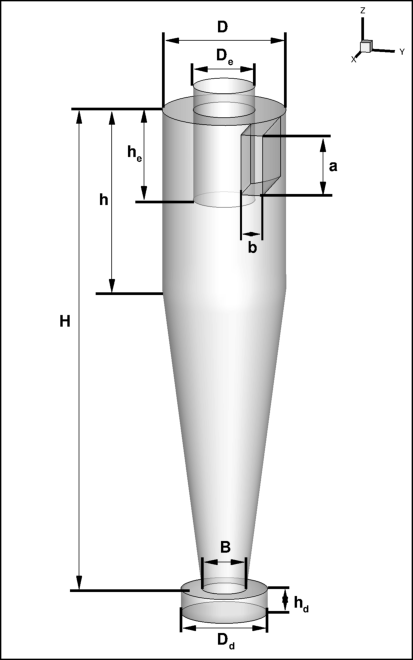
\includegraphics[scale=0.5]{Geometry}
				\captionof{figure}{Схема фильтра}
  \end{minipage}
%Решение
\newpage
\begin{thebibliography}{9}

\bibitem{openfoam} Официальный сайт OpenFOAM, \url{http://www.openfoam.com}
\bibitem{Monson} Monson, D. J., Seegmiller, H. L., Mc Connaughey, P. K., and Chen, Y. S., “Comparison of Experiment With Calculations Using Curvature-Corrected Zero and Two Equation Turbulence Models for a Two-Dimensional U-Duct”, AIAA Paper No. 90-1484, 1990.
\bibitem{emissionInfoRussian} Загрязнение окружающей среды в субъектах РФ, \url{http://protown.ru/information/hide/2659.html}
\bibitem{emissionInfoEurope} A. Wilson, “Cement and Concrete: Environmental Considerations”, EBN Volume 2, No. 2, 1993
\bibitem{DirgoLeith} J. Dirgo, D. Leith, “Cyclone collection efficiency: comparison of experimental results with theoretical predictions”, Aerosol Sci. Tech. 4 410–415, 1985.
\bibitem{instructions} Ужов В.Н. Циклоны НИИОГАЗ. Руководящие указания по проектированию, изготовлению, монтажу и эксплуатации. Ярославль, 1970
\bibitem{Menter} Menter, F., Esch, T. “Elements of Industrial Heat Transfer Prediction”, 16th Brazilian Congress of Mechanical Engineering (COBEM), Nov. 2001
\bibitem{OPNFPG} OpenFOAM Programmer’s Guide, 2011
\end{thebibliography}
\end{document}
